\chapter{Diseño e implementación} % Main chapter title

\label{Chapter3} % Change X to a consecutive number; for referencing this chapter elsewhere, use \ref{ChapterX}
Durante este capítulo se explica el diseño e implementación del software y hardware del equipo. También se detalla y justifica el motivo de las implementaciones realizadas.

\section{Diseño del Hardware}
\subsection{Cruce por cero}

Debido a que la medición de una descarga parcial debe estar relacionada con la senoide de referencia por medio de su momento angular, el equipo fue provisto de un medio para conocer esta variable del sistema de forma constante.

El método elegido para la medición de fase fue un circuito de detección de cruce por cero combinado con un timer interno del microcontrolador. Se optó por este método porque puede ser aislado por medio de un optoacoplador y soportar conexiones directas con senoides de referencia de hasta 300 V. Otro motivo es que solo al ser de interés el momento angular, un timer de 32 bits brinda mejor resolución que un conversor analógico digital y requiere menos procesamiento.

El circuito diseñado, figura \ref{fig:schZeroCross}, está basado en un optocoplador LTV357 \citep{opto:ltv357}. Este presenta una aislación de 3750 Vrms entre entrada y salida. La polarización del led de entrada se realizó por medio de un C8 y tiene un rango dinámico de tensión de entrada entre 50 Vpp y 340 Vpp. 

\begin{figure}[ht]
	\centering
	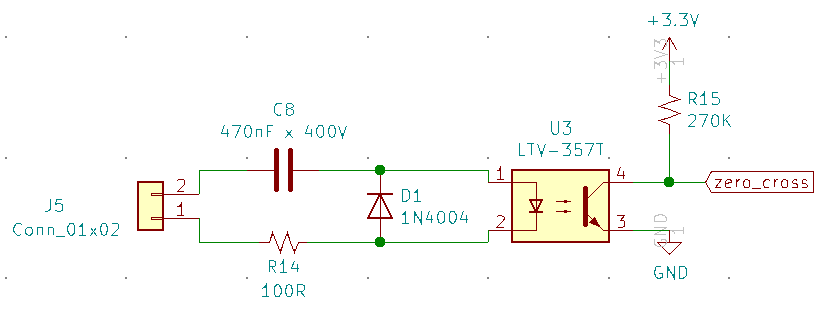
\includegraphics[width=130mm]{./Figures/schZeroCross.png}
	\caption{Entrada de detección de cruce por cero para la senoide de referencia.}
	\label{fig:schZeroCross}
\end{figure}

\newpage

El cálculo del valor de C8 fue determinado por la corriente de polarización del led (\textit{If}), la corriente de colector (\textit{Ic}) y la relación de transferencia (CTR), figura \ref{fig:ltvCtr}.  

\begin{figure}[ht]
	\centering
	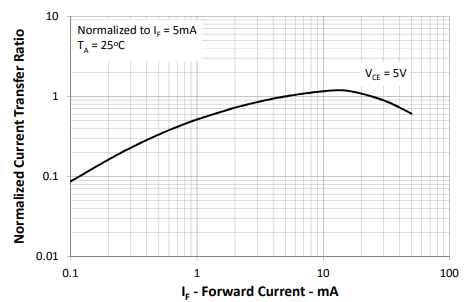
\includegraphics[width=130mm]{./Figures/ltvCtr.png}
	\caption{Relacion de transferencia del LTV357.}
	\label{fig:ltvCtr}
\end{figure}

En base a la curva \ref{fig:ltvCtr}, se calculó la corriente mínima necesaria \textit{If} para polarizar el transistor del optoacoplador. Para este cálculo se consideró como tensión mínima de polarización a una senoide de 50 Vpp luego de haber transcurrido 1 grado desde su cruce por cero. Esto se debe a que la resolución mínima deseada del equipo es 1 grado y por lo tanto el circuito debe detectar el cruce por cero dentro de este periodo.

En la tabla \ref{tab:corriente} se observa que la corriente \textit{If} máxima en 340 Vpp no excede los 50 mA y que la corriente \textit{Ic} mínima en 50 Vpp es superior a los 0,0122 mA necesarios para polarizar el circuito.

\vspace{5mm}

\begin{table}[h]
\centering
\caption[Corrientes de polarización]{Corrientes de polarización}
\begin{tabular}{l c c c c}
\toprule
\textbf{Vpp} & \textbf{If(mA) @ 1°} & \textbf{Ic(mA) @ 1°} & \textbf{If(mA) @ 90°} & \textbf{Ic(mA) @ 90°}\\
\midrule
340 & 0,88 & 0,35 & 50,2 & 30,12 \\
50 & 0,13 & 0,0129 & 7,38 & 7,38\\
\bottomrule
\hline
\end{tabular}
\label{tab:corriente}
\end{table}

\vspace{5mm}

El optoacoplador elegido solo posee un LED que se polariza durante un semiciclo. Esto permite reconocer de forma sencilla el semiciclo positivo y negativo. El diodo D1 protege al LED interno del optoacoplador cuando se encuentra en polarizado inversa.

La salida del circuito se encuentra conectada a un pin del microcontrolador que permite el mapeo de interrupciones externas.

\vspace{10mm}
\subsection{Filtro}

Para la medición de la descarga parcial se utilizó el conversor analógico digital de alta velocidad del LPC4370 \citep{micro:lpc4370}, configurado en modo diferencial. En el capítulo 2 se explicó la importancia de un filtro \textit{anti-aliasing} para evitar interferencia de frecuencias indeseadas en la medición. Ya que el conversor analógico digital tiene una velocidad máxima de 80 MSPS, el filtro fue calculado para tener una frecuencia de corte igual a 40MHz. Figura \ref{fig:respFrec}. 

\begin{figure}[ht]
	\centering
	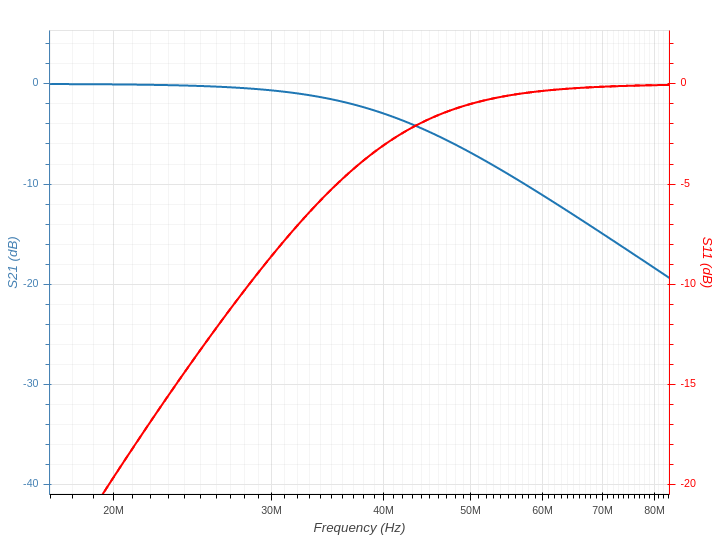
\includegraphics[width=130mm]{./Figures/respFrec.png}
	\caption{Respuesta en frecuencia deseada.}
	\label{fig:respFrec}
\end{figure}


El filtro implementado es un filtro \textit{Butterworth} diferencial de 3er orden con una atenuación de -3dB en 40 MHz, figura \ref{fig:schFiltro}. El ingreso de la señal al filtro se realiza por medio de dos capacitores de desacople y un transformador 1:1, esto permite conectar un sensor inductivo en modo común o diferencial. 

\begin{figure}[ht]
	\centering
	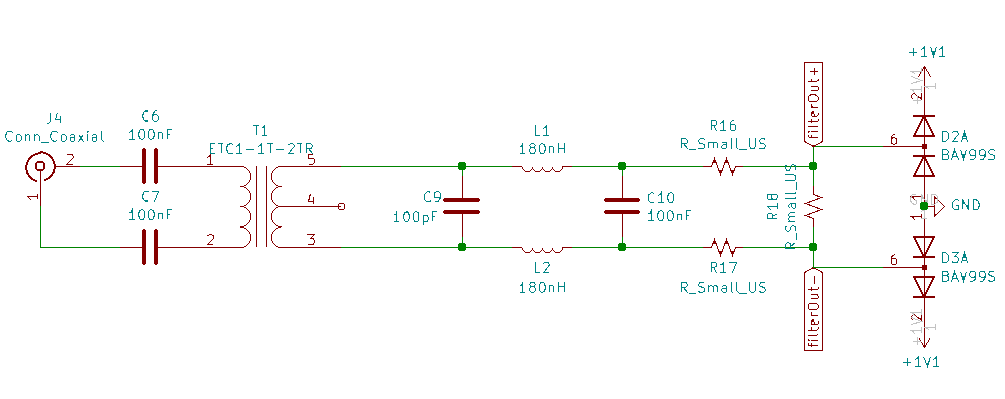
\includegraphics[width=140mm]{./Figures/schFiltro.png}
	\caption{Filtro diferencial \textit{Butterworth} de 3er orden. Frecuencia de corte 40Mhz.}
	\label{fig:schFiltro}
\end{figure}


Puede observarse que al final del filtro se incluye un divisor resistivo y un enclavamiento de diodos para proteger al periférico de sobretensiones. El divisor permite atenuar linealmente la señal en caso de requerir mayor rango dinámico de entrada y también podría servir en caso de requerir agregar una etapa más al filtro.

\subsection{Esquemático general} 

El módulo central es el microprocesador LPC4370, figura \ref{fig:schCentral}. A este llegan la señal analógica proveniente del filtro diferencial y la entrada aislada de la detección del cruce por cero. Pueden observarse los componentes necesarios para el funcionamiento reloj de tiempo real (RTC), estos son un cristal de 32 KHz y una batería.


\begin{figure}[ht]
	\centering
	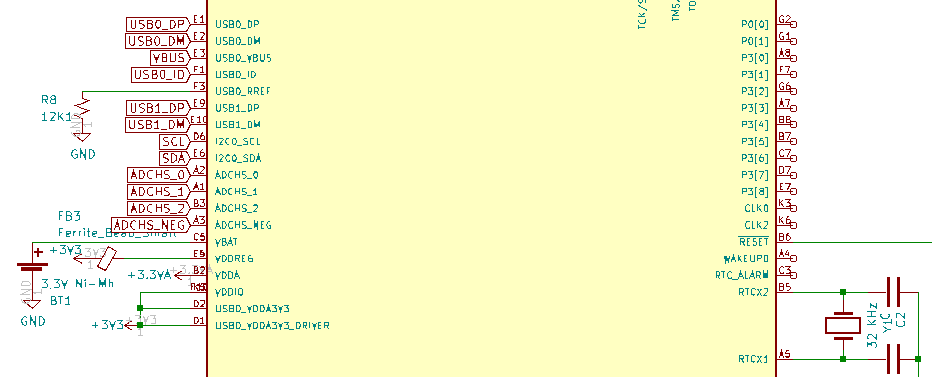
\includegraphics[width=140mm]{./Figures/schCentral.png}
	\caption{Procesador y RTC.}
	\label{fig:schCentral}
\end{figure}


\subsection{Fuente}

La fuente de alimentación, figura \ref{fig:schPwr}, fue diseñada por medio de dos reguladores lineales. Se utilizó el regulador de 3,3 V junto con dos filtros PI para generar dos ramas, una para los módulos digitales y otra los módulos analógicos. El regulador de 1,1 V cumple la función de generar la tensión de enclavamiento para el circuito de protección de la etapa analógica.


\begin{figure}[ht]
	\centering
	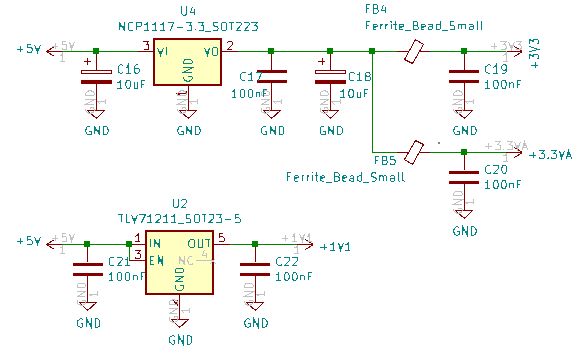
\includegraphics[width=110mm]{./Figures/schPwr.png}
	\caption{Fuentes de alimentación.}
	\label{fig:schPwr}
\end{figure}

\vspace{5mm}

\subsection{Comunicaciones}

Como periféricos de comunicación se proporcionó un puerto 232, figura \ref{fig:schSerial}, para acceder a la interfaz del sistema. 

\begin{figure}[ht]
	\centering
	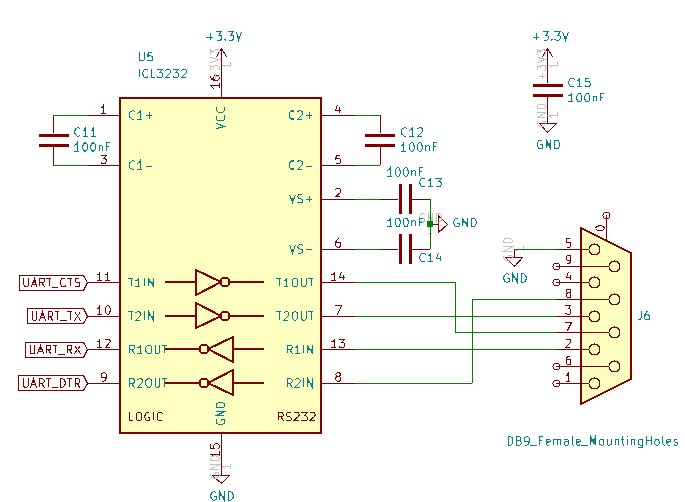
\includegraphics[width=95mm]{./Figures/schSerial.png}
	\caption{Circuito de comunicacion serial.}
	\label{fig:schSerial}
\end{figure}

También se incluyeron dos puertos USB de alta velocidad, figura \ref{fig:schUSB}, uno para conexión directa de un pendrive y otro para conexión \textit{on-the-go} para futuras opciones.

\begin{figure}[ht]
	\centering
	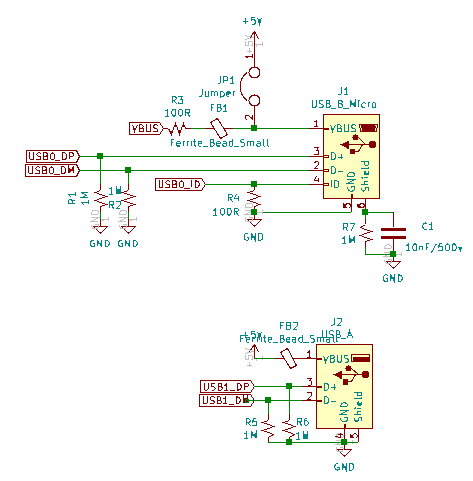
\includegraphics[width=90mm]{./Figures/schUSB.png}
	\caption{Circuitos de comunicacion USB.}
	\label{fig:schUSB}
\end{figure}

\newpage

\section{Diseño del Firmware}

Si bien el LPC4370 dispone de tres núcleos, este trabajo se realizó utilizando solo el cortex M4 dejando libres los dos cortex M0. De esta forma quedan recursos disponibles para implementar futuros procesamientos de la señal. 

Inicialmente se había planificado utilizar un sistema operativo de tiempo real, pero se descartó debido a que la ejecución de tareas durante el proceso de disparo del \textit{trigger} generan \textit{jitter} al comienzo de la adquisición. 

Las soluciones planteadas para este problema fueron:
\vspace{5mm}

\begin{itemize}
\item detener el scheduler en momentos específicos.
\item portar el kernel de freertos tickless para este procesador.
\item evitar el uso de un sistema operativo y realizar el software bajo el patrón de software \textit{superpoll}.
\end{itemize}   

\vspace{5mm}

Por ser una solución de menor complejidad y debido al tiempo disponible para realizar el trabajo, la última alternativa fue la elegida.

El firmware fue desarrolado en lenguaje C y se dividió en varios módulos funcionales que encapsulan su comportamiento, figura \ref{fig:firmBloques}. La interacción entre los módulos se realizó por medio de funciones públicas utilizadas como interfaces. 
\vspace{10mm}

\begin{figure}[ht]
	\centering
	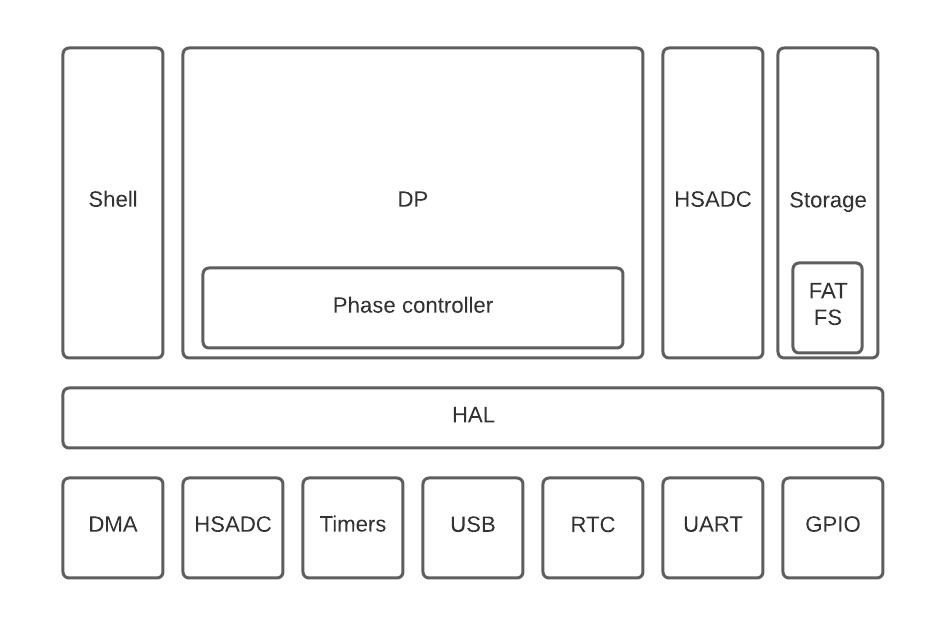
\includegraphics[width=140mm]{./Figures/firmBloques.png}
	\caption{Diagrama en bloques de los módulos de firmware.}
	\label{fig:firmBloques}
\end{figure}


\subsection{Shell}
El equipo dispone de una interfaz de usuario desarrollada para funcionar en cualquier terminal estándar de 80 caracteres por línea. Esta es accesible por medio de un puerto serial bajo una configuración 115200,8,n,1.

La interfaz permite configurar el equipo, realizar, navegar y visualizar mediciones. Los comandos se componen de una palabra principal y en algunos casos permiten parámetros adicionales. 

\vspace{5mm}

Existen 4 grupos de comandos:
\begin{itemize}
\item  de configuración.
\item  de navegación.
\item  de visualización.
\item de estado. 

\end{itemize}

\vspace{5mm}

Breve descripción de los comandos:
\begin{itemize}
\item mode -a [m]: permite activar el modo de adquisición automático con un intervalo de tiempo [minutos]. Este modo inicializa la creación de un patrón de DP cada \textit{m} minutos.
\item mode -i [g-p] : inicializa la creación de un patrón de DP. Con el parámetro [g] lo grafica por medio de caracteres ASCII y no es guardado. Con el parámetro [p] el patrón y el muestreo de las descargas parciales son guardados en el pendrive.
\item mode -d : desarma el trigger y en caso de haber un patrón de DP en proceso de creación lo guarda.
\item dccal: calibración para eliminar componente de continua.
\item conf -t [mV] : permite configurar el valor del trigger en [mV]. El mismo valor será considerado como absoluto y será establecido como trigger positivo y negativo.
\item conf -q [puntos] : permite configurar la cantidad de puntos (DP) que constituirán un patrón de DP (hasta 1500). 
\item conf -s [muestras] : permite configurar la cantidad de muestras por DP (hasta 968).
\item time -g : imprime el valor de fecha y hora en pantalla bajo el formato hh:mm:ss DD/MM/AAAA.
\item time -s [hh:mm:ss DD/MM/AAAA]: permite configurar la fecha y hora.
\item lspd : lista todos los patrones de DP existentes en el pendrive.
\item lspd -f [AAAAMMDDhhmm]:  lista los patrones existentes en el pendrive y los filtra según el año (AAAA), mes (MM), día (DD), horas (hh), minutos (mm) y segundos (ss) ingresados. Cualquier atributo puede reemplazarse por el caracter ‘?’ para ignorar el filtro.
\item dwnpd -g [AAAAMMDDhhmm] : permite graficar por medio de caracteres ASCII el patrón de descargas parciales seleccionado.
\item dwnpd -t [AAAAMMDDhhmm] : permite enviar en forma de tabla el patrón seleccionado.
\item restart : reinicia el cpu.
\item info -s : brinda información sobre el sistema
\item ?: información sobre los comandos.
\end{itemize}

\vspace{5mm}

La interfaz dispone de un modo de visualización de patrones de descarga parcial generado por caracteres \textit{ASCII}, figura \ref{fig:firmInterfaz}. Debido a la baja resolución existente en este modo, se utilizaron diferentes caracteres para representar densidad de DP en un área del patrón determinada. Este modo es especialmente práctico para configuración o consultas remotas. También puede solicitarse que una DP sea visualizada en forma de tabla.

\vspace{5mm}

\begin{figure}[ht]
	\centering
	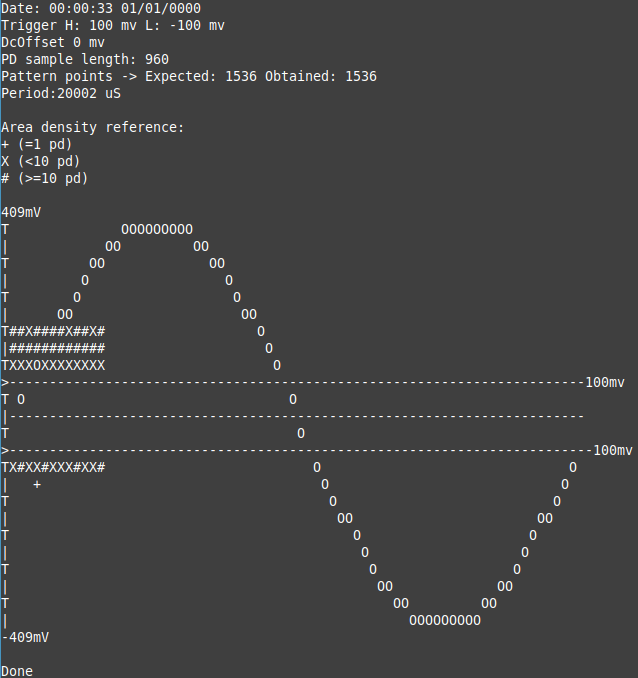
\includegraphics[width=130mm]{./Figures/firmInterfaz.png}
	\caption{Patrón de DP por terminal.}
	\label{fig:firmInterfaz}
\end{figure}

Los archivos almacenados en el pendrive por cada patrón de DP son tres, figura \ref{fig:firmFiles}. Un archivo \enquote{.info} que contiene los parámetros de la medición realizada, un archivo \enquote{.mem} que contiene los datos crudos con las formas de onda de las DP y un archivo \enquote{.csv}. Este último archivo puede ser abierto por cualquier planilla de cálculo y contiene el patrón de DP representado por los conjuntos \enquote{pico-fase}.

\vspace{5mm}

\begin{figure}[ht]
	\centering
	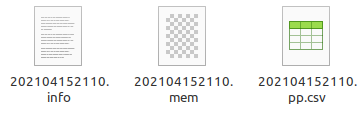
\includegraphics[width=60mm]{./Figures/firmFiles.png}
	\caption{Archivos generados como resultado de la creación de un patrón.}
	\label{fig:firmFiles}
\end{figure}

\subsection{DP}

Dentro de este módulo se realiza el control de las adquisiciones de DP, el posterior procesamiento y conformación del patrón. Este es el módulo central, funciona como consumidor de las funciones que implementan los demás módulos.

Dentro de este módulo tambien se realiza el control de fase. La detección de cruce por cero es realizada por una interrupción por hardware configurada por flanco ascendente. En la rutina de interrupción se inicia un timer que se encarga de medir el tiempo de forma constante entre cruces. Consultando este timer en cualquier momento y desde cualquier parte del código, puede conocerse por regla de tres simple la fase de la senoide de referencia. En la figura \ref{fig:firmFSM} puede verse el diagrama de la máquina de estado encargada de controlar el momento angular.

\begin{figure}[ht]
	\centering
	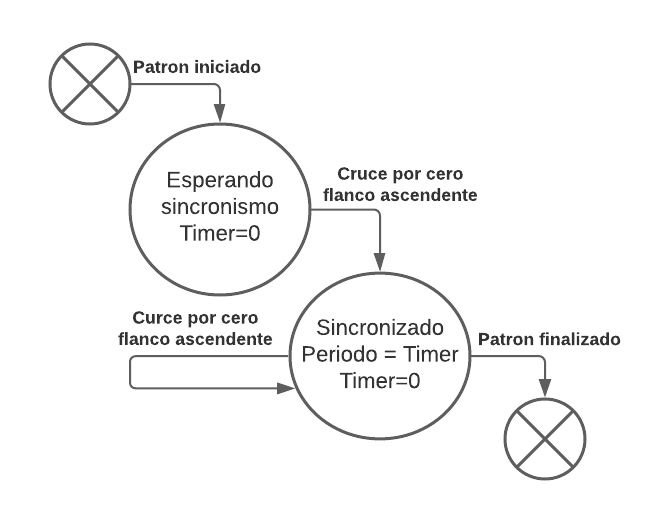
\includegraphics[width=100mm]{./Figures/firmZCFSM.png}
	\caption{FSM control de fase.}
	\label{fig:firmFSM}
\end{figure}

\newpage

\subsection{HSADC}

La gestión de memoria interna fue una pieza clave para el correcto funcionamiento del sistema. El conversor analógico digital junto con su acceso directo a memoria (DMA) generan muestras de 12 bits a una tasa de 80 MHz. Debido a la arquitectura del cortex M4, los accesos al mismo banco de memoria no pueden realizarse de forma simultánea. Para asegurar que no se pierdan muestras de la adquisición, se asignó al periférico ADC un banco de memoria exclusivo, figura \ref{fig:firmMemoria}.

\begin{figure}[ht]
	\centering
	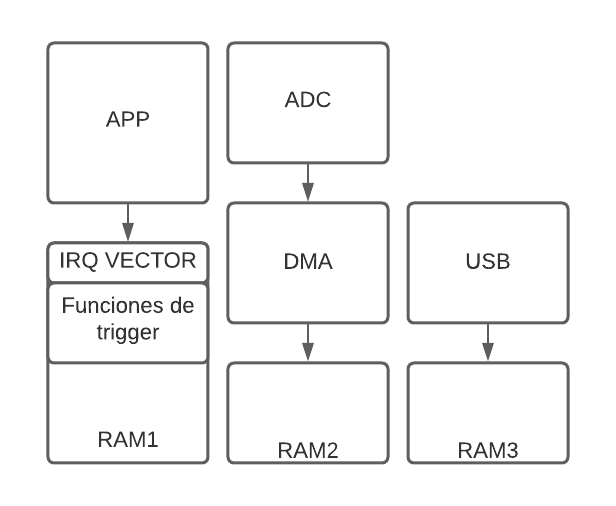
\includegraphics[width=110mm]{./Figures/firmMemoria.png}
	\caption{Diagramas de bloque general de distribución de memoria.}
	\label{fig:firmMemoria}
\end{figure}

Un disparo de \textit{trigger} se realiza por medio de una comparación entre una muestra y un umbral establecido previamente. Para poder realizar esta comparación, el periférico necesita adquirir muestras constantemente, esto genera un flujo de datos que debe administrarse. Para resolver esto se utilizó una cola circular en memoria en donde el DMA copia los datos adquiridos de forma constante y elimina siempre la muestra más antigua. Cuando el \textit{trigger} es disparado se almacena el puntero a la posición inicial y cuando la cola completa la vuelta se finaliza la adquisición. El resultado es una ventana de \textit{N} muestras que puede ser propagada a otras capas de software para su correcta manipulación. 

Por practicidad, el modulo de firmware HSADC administra su memoria como un único banco, figura \ref{fig:firmBanco}, este banco a su vez es dividido en \textit{slots}. Todos los slots son de igual tamaño y permiten adquirir ininterrumpidamente a partir de un disparo de trigger. Una vez concluida la adquisición del \textit{slot},  en caso de quedar slots libres, el sistema se rearma y queda a la espera de un próximo disparo. En caso de haber completado todos los \textit{slots} del banco de memoria, se procesa y almacena.

\begin{figure}[ht]
	\centering
	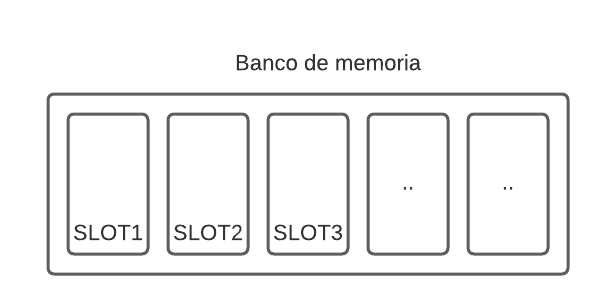
\includegraphics[width=100mm]{./Figures/firmBanco.png}
	\caption{Banco de memoria.}
	\label{fig:firmBanco}
\end{figure}

\newpage

\subsection{Storage}

Este módulo se encarga de encapsular el funcionamiento del pendrive y su sistema de archivos. Implementa el sistema de archivos FAT32 por medio de la librería FatFs \citep{chanWeb:1} combinado con los drivers USB provistos por NXP.


\section{Herramientas de usuario}

Para dar mayor capacidad de análisis sobre las mediciones adquiridas se desarrollaron dos scripts en Python3 que procesan los datos almacenados en el pendrive. 
\begin{itemize}
\item El primero permite generar un patrón de DP de forma gráfica a partir de una archivo \enquote{.csv}.
\item El segundo permite reconstruir las señales obtenidas de cada DP a partir de una archivo \enquote{.mem} y generar un gráfico por cada una.
\end{itemize}  

\vspace{5mm}

\begin{figure}[ht]
	\centering
	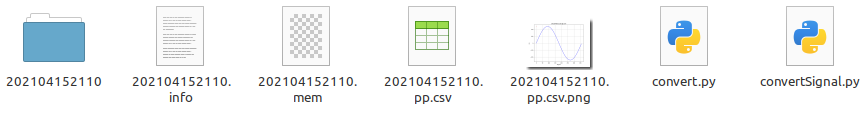
\includegraphics[width=140mm]{./Figures/firmAllFiles.png}
	\caption{Árbol completo de archivos luego del procesamiento con scripts.}
	\label{fig:firmAllFiles}
\end{figure}

\section{Prototipo funcional}

Un prototipo funcional fue montado como validador tecnológico y a su vez para poder llevar a cabo los ensayos. El mismo fue construido utilizando una placa de desarrollo \enquote{LPC link2}, figura \ref{fig:hardLPC}. A pesar de no estar disponibles todos los pines del microprocesador, la placa fue modificada para poder acceder a todos los periféricos requeridos en este trabajo. La única restricción encontrada fue el acceso a la alimentación independiente del reloj de tiempo real, lo cual hace que en este prototipo la fecha y hora se pierda siempre que falte el suministro eléctrico. 

\begin{figure}[ht]
	\centering
	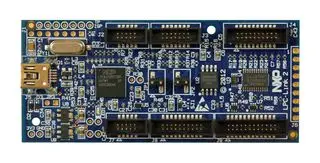
\includegraphics[width=100mm]{./Figures/hardLPC.png}
	\caption{LPC link2.}
	\label{fig:hardLPC}
\end{figure}

\vspace{10mm}

Como tareas de modificación se removieron los filtros existentes en modo común de las entradas analógicas para que no afecten a los nuevos filtros diferenciales conectados. Tambien se agregó un cristal de 32 KHz como oscilador del reloj de tiempo real.

La placa de desarrollo solo dispone de un puerto USB diseñado para ser utilizado como device y ser conectado a la PC. El circuito fue modificado para funcionar como host y ser alimentado desde la fuente. También se utilizó un adaptador micro USB a USB A para poder conectar un pendrive.  

Para finalizar el prototipo funcional, figura \ref{fig:hardProto}, se agregó una placa adicional con el filtro diferencial y la etapa de optoacoplado. La conexiones entre los dos circuitos impresos fueron realizadas por medio de los puertos de expansión del \enquote{LPC link2}. 

\vspace{10mm}

\begin{figure}[ht]
	\centering
	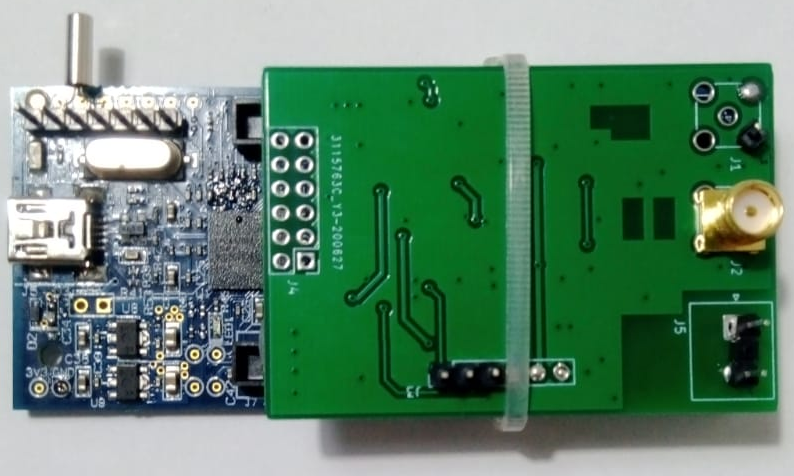
\includegraphics[width=100mm]{./Figures/hardProto.png}
	\caption{Prototipo funcional.}
	\label{fig:hardProto}
\end{figure}